\documentclass{uc3mpracticas}

\usepackage{helvet}
\usepackage{multicol}
\renewcommand{\familydefault}{\sfdefault}
\usepackage{changepage}
\usepackage{geometry}
\usepackage{caption}
\usepackage{xcolor,colortbl}

\definecolor{Gray}{gray}{0.85}
\definecolor{LightCyan}{rgb}{0.88,1,1}
\definecolor{LightGreen}{rgb}{0.29,1,0.39}

\newcolumntype{g}{>{\columncolor{Gray}}l}

%%%%%%%%%%%%%%%%%%%%%%%%%%%%%%%%%%%%%%%%%%%%%%%%%%%%%%%%%%%%%%%%%%%%%%%%%%%%%%%%
%%%                   Plantilla Prácticas UC3M                               %%%
%%%                Universidad Carlos III de Madrid                          %%%
%%%                   Alejandro Valverde Mahou                               %%%
%%%%%%%%%%%%%%%%%%%%%%%%%%%%%%%%%%%%%%%%%%%%%%%%%%%%%%%%%%%%%%%%%%%%%%%%%%%%%%%%

%Permitir cabeceras y pie de páginas personalizados
\pagestyle{fancy}

%Path por defecto de las imágenes
\graphicspath{ {./images/} }

%Declarar formato de encabezado y pie de página de las páginas del documento
\fancypagestyle{doc}{
  %Cabecera
  \headerpr[1]{Problema de Clasificación: Parte I}{}{Redes de Neuronas Artificiales}
  %Pie de Página
  \footerpr{}{\textbf{UC3M}}{{\thepage} de \pageref{LastPage}}
}

%Declarar formato de encabezado y pie del título e indice
\fancypagestyle{titu}{%
  %Cabecera
  \headerpr{}{}{}
  %Pie de Página
  \footerpr{}{}{}
}


\appto\frontmatter{\pagestyle{titu}}
\appto\mainmatter{\pagestyle{doc}}


\begin{document}
  %Comienzo formato título
  \frontmatter


  %Portada 1 (Centrado todo)
  \centeredtitle{Images/LogoUC3M.png}{Grado en Ingeniería Informática}{Curso 2020/2021}{Redes de Neuronas Artificiales}{Problema de Clasificación: Parte I}{Clasificación de imágenes del cielo con el Perceptrón Multicapa}

  \vspace{55mm}

  \authors{Alba Reinders Sánchez}{100383444}{Alejandro Valverde Mahou}{100383383}{}{}{}{}

  \newpage

  %Índice
  \tableofcontents

  \newpage

  %Comienzo formato documento general
  \mainmatter

\section{Introducción}

El problema planteado consiste en clasificar imágenes del cielo con el objetivo de ayudar a la estimación de la radiación solar que incide en un lugar, ya que la cantidad de esta radiación varía si hay nubes o no, y del tipo de las nubes.

\vspace{3mm}

Para ello, se hace una simplificación del problema real reduciendo a tres posibles clases las imágenes:

\begin{itemize}
  \item Cielo Despejado: \textit{48 ejemplos}
  \item Nube \textit{(sólo un tipo de nube)}: \textit{513 ejemplos}
  \item Multinube \textit{(varios tipos de nube)}: \textit{156 ejemplos}
\end{itemize}

Dado que en esta primera parte de la práctica se trabaja con un \textbf{Perceptrón Multicapa}, es necesario transformar la información de la imagen en distintos atributos numéricos.

\vspace{3mm}

Los datos que se usan en esta práctica provienen del \textit{grupo MATRAS de la Universidad de Jaén} y contienen estadísticos y transformaciones de imágenes del cielo completo, que permiten al Perceptrón Multicapa realizar la clasificación.

\vspace{2mm}

El conjunto de datos tiene \textbf{717} instancias con \textbf{12} atributos de entrada y \textbf{1} atributo de salida, la clase.

\begin{enumerate}
  \begin{multicols}{2}
  \item Media del canal azul
  \item Media del canal rojo
  \item Desviación típica del canal azul
  \item Sesgo del canal azul
  \item Diferencia de medias Rojo – Verde
  \item Diferencia de medias Rojo – Azul
  \columnbreak
  \item Diferencia de medias Verde – Azul
  \item Entropía del canal azul
  \item Energía del canal azul
  \item Contraste del canal azul
  \item Homogeneidad del canal azul
  \item Cobertura
  \end{multicols}
\end{enumerate}



\section{Preparación de los datos}

Se debe hacer un preprocesado de los datos para poder realizar de manera más efectiva el entrenamiento de la red. Primero se normaliza el conjunto de datos y después se divide en 4 subconjuntos, ya que se lleva a cabo \textit{validación cruzada estratificada} de 4 hojas.

\subsection{Normalizar}

Es necesario normalizar los datos de entrada, dado que cada atributo suele tener rangos de valores muy diferentes. Normalizarlos en el intervalo [0,1] evita posibles sesgos generados por esta difencia de rangos de los atributos durante el aprendizaje de la red.


\subsection{Preparar los datos para Validación Cruzada Estratificada}

Se realiza esta técnica debido a que las clases están desbalanceadas, por tanto no se puede aplicar la validación cruzada normal y se tiene que llevar a cabo la \textit{estratificada}.

\vspace{2mm}

Para realizar la división de los datos en 4 hojas que mantengan la proporción de instancias de las 3 clases, se crean 4 subconjuntos de las instancias de cada clase y después se junta un subconjunto de cada clase en cada hoja.

\vspace{2mm}

Una vez se tienen las 4 hojas, se crean 4 parejas de ficheros para componer los datos de entrenamiento y test. Combinando las distintas hojas de distinta forma, dejando siempre una para el test. Por último se aleatorizan los datos de entrenamiento para evitar posibles sesgos.



\section{Experimentación y análisis de resultados}

La experimentación con el \textit{Perceptrón Multicapa} se basa en ir haciendo experimentos de manera progresiva intentado conseguir la mejor configuración posible, de forma que tanto el error de entrenamiento como el error de test sea mínimo. Además, dado que las clases no están balanceadas, se tiene que tener en cuenta a su vez el porcentaje de aciertos, siendo esta última medida sobre el conjunto de test la que se va a usar como determinante para decidir qué configuración es mejor que otra.

\vspace{2mm}

 Para ello se van variando los hiperparámetros de la red: la \textbf{topología} de la red, la \textbf{razón de aprendizaje} (\textit{RA}) y el \textbf{número ciclos máximo}. Los distintos experimentos que se crean mantienen la topología pero se va modificando la \textit{RA} que se utiliza.

\vspace{1mm}

Los resultados que se muestran en las distintas tablas son las medias de resultados de las 4 hojas de la \textit{validación cruzada estratificada}. Destacar que el \textbf{número de ciclos máximos} se fija a \textbf{10000} en un primer momento, y se probará a modificarlo más adelante.


\begin{figure}[!h]
\begin{center}
  \begin{tabular}{|c|c|c|}
    \hline
    \rowcolor{Gray}
                  \textbf{Configuración}                        & \textbf{\% de aciertos entrenamiento} & \textbf{\% de aciertos test}\\ \hline \hline
        \rowcolor{LightGreen}
        \textit{\textbf{c(10), RA=0,001}} &  0,7629008897                         &  0,6738700565               \\ \hline
        \textit{\textbf{c(10), RA=0,007}} &  0,3823117112                         &  0,3219868173               \\ \hline
        \textit{\textbf{c(10), RA=0,01}}  &  0,839641527                          &  0,6432438795               \\ \hline
        \textit{\textbf{c(10), RA=0,005}} &  0,7991775295                         &  0,6474811676               \\ \hline \hline \hline

        \textit{\textbf{c(100), RA=0,001}}&  0,7643001241                         &  0,6627354049               \\ \hline
        \textit{\textbf{c(100), RA=0,005}}&  0,8001163873                         &  0,6613700565               \\ \hline
        \rowcolor{LightGreen}
        \textit{\textbf{c(100), RA=0,0008}}&  0,7582428098                         &  0,6669256121               \\ \hline
        \textit{\textbf{c(100), RA=0,0006}}&  0,7521984275                         &  0,5525188324               \\ \hline \hline \hline

        \textit{\textbf{c(10,10), RA=0,001}}&  0,3692892613                         &  0,2372175141               \\ \hline
        \rowcolor{LightGreen}
        \textit{\textbf{c(10,10), RA=0,01}}&  0,851228533                         &  0,6447975518               \\ \hline
        \textit{\textbf{c(10,10), RA=0,03}}&  0,9432547072                         &  0,6235640301               \\ \hline
        \textit{\textbf{c(10,10), RA=0,008}}&  0,8307702255                         &  0,6433145009               \\ \hline \hline \hline

        \textit{\textbf{c(10,10,10), RA=0,001}}&  0,06694599628                         &  0,06694915254               \\ \hline
        \rowcolor{LightGreen}
        \textit{\textbf{c(10,10,10), RA=0,01}}&  0,8191754604                         &  0,6962806026               \\ \hline
        \textit{\textbf{c(10,10,10), RA=0,008}}&  0,6734171322                         &  0,5252118644               \\ \hline \hline \hline

        \textit{\textbf{c(10,10,10,10), RA=0,001}}&  0,06694599628                        &  0,06694915254               \\ \hline
        \textit{\textbf{c(10,10,10,10), RA=0,01}}&  0,06694599628                         &  0,06694915254               \\ \hline
        \rowcolor{LightGreen}
        \textit{\textbf{c(10,10,10,10), RA=0,02}}&  0,1727989861                         &  0,1692561205               \\ \hline
  \end{tabular}
\end{center}
\caption*{Tabla resumen con el porcentaje de aciertos de media en entrenamiento y test}
\end{figure}



\subsection{Experimento 1}

Es el caso base desde el que se parte, se tiene \textbf{una única capa oculta con 10 neuronas}. A continuación en la tabla se muestra los resultados obtenidos para las distintas razones de aprendizaje.

\begin{figure}[!h]
\begin{center}
  \begin{tabular}{|c|c|c|c|c|}
    \hline
    \rowcolor{Gray}
        \textit{\textbf{RA}}  & \textbf{Error entrenamiento} & \textbf{\% de aciertos entrenamiento} & \textbf{Error test} & \textbf{\% de aciertos test}\\ \hline
        \rowcolor{LightGreen}
        \textit{0,001}        &  \textit{0,3344952944}       &  \textit{0,7629008897}                & \textit{0,4235530262}& \textit{0,6738700565}      \\ \hline
        0,0007                &  0,3549707553                &  0,3823117112                         &  0,4343040342       &  0,3219868173               \\ \hline
        0,01                  &  0,2505371572                &  0,839641527                          &  0,4613691504       &  0,6432438795               \\ \hline
        0,005                 &  0,2792817569                &  0,7991775295                         &  0,4438048242       &  0,6474811676               \\ \hline

  \end{tabular}
\end{center}
\caption*{Tabla resultados Experimento 1}
\end{figure}

Los resultados que se obtienen no son muy prometedores, partiendo del primer subexperimento (se denominará como el original) con \textit{RA} de \textit{0,001}, se intenta ir aumentando o disminuyendo su valor en los siguientes subexperimentos para encontrar la mejor \textit{RA} para esta topología. Después de probar con diferentes valores, se concluye con que la mejor \textit{RA} es la original: \textit{0,001}.

\vspace{2mm}

Se ha podido observar que cuando se disminuye la \textit{RA} los errores son similares pero el porcentaje de aciertos, tanto en entrenamiento como en test disminuye prácticamente a la mitad. Esto puede deberse a que en la mayoría de casos está prediciendo la clase mayoritaria (\textbf{nube}), lo cuál hace que el modelo tenga un error que no es del todo malo, pero el porcentaje de aciertos, como es de esperar, es malo.

\vspace{1mm}

Por otro lado, al aumentar la \textit{RA}, en entrenamiento el error disminuye y el porcentaje de aciertos aumenta, lo que puede ser una buena señal. Pero en test el error aumenta y el porcentaje de aciertos disminuye, lo cuál indica un sobreaprendizaje, haciendo que estos modelos sean peores que el original. Aún así, el modelo original muestra también un claro sobreaprendizaje, lo que se intentará reducir en los siguientes experimentos.


\subsection{Experimento 2}

Al igual que en el experimento anterior, se tiene una única capa oculta pero se aumenta el \textbf{número de neuronas a 100} para comprobar si esto afecta positivamente a los resultados. Los resultados obtenidos para las distintas razones de aprendizaje son:

\begin{figure}[!h]
\begin{center}
  \begin{tabular}{|c|c|c|c|c|}
    \hline
    \rowcolor{Gray}
        \textit{\textbf{RA}}  & \textbf{Error entrenamiento} & \textbf{\% de aciertos entrenamiento} & \textbf{Error test} & \textbf{\% de aciertos test}\\ \hline
        0,001                 &  0,3410726584                &  0,7643001241                         &  0,4513887673       &  0,6627354049               \\ \hline
        0,005                 &  0,2828611825                &  0,8001163873                         &  0,4455312415       &  0,6613700565               \\ \hline
        \rowcolor{LightGreen}
        \textit{0,0008}       &  \textit{0,3488769075}       &  \textit{0,7582428098}                &  \textit{0,4522441869}&  \textit{0,6669256121}               \\ \hline
        0,0006                &  0,3566408764                &  0,7521984275                         &  0,4524900392       &  0,5525188324               \\ \hline

  \end{tabular}
\end{center}
\caption*{Tabla resultados Experimento 2}
\end{figure}

Tal y como se ve en la tabla, el aumentar el número de neuronas no ha hecho que los resultados mejoren. Primero se aumenta la \textit{RA}, y en este caso, los valores son muy similares al caso original con \textit{0,001} de \textit{RA}.

\vspace{2mm}

Dado que aumentar la \textit{RA} no genera mejores resultados, se prueba a disminuirla. El tercer subexperimento proporciona mejores resultados en el conjunto de test, por lo que se prueba a disminuir todavía más, pero esto empeora los resultados.

\vspace{1mm}

Por tanto, el mejor subexperimento para la topología de este experimento es el que tiene una \textit{RA} de \textit{0,0008}. Sin embargo, no se observa una mejora respecto al mejor del \textbf{Experimento 1}, por lo que se puede concluir que aumentar el número de neuronas con una única capa no genera un cambio significatvo.


\subsection{Experimento 3}

En este caso se aumenta el \textbf{número de capas ocultas a 2, con 10 neuronas cada una}. Se intenta probar si una topología algo más compleja obtiene mejores resultados. Los resultados obtenidos para las distintas razones de aprendizaje son:

\begin{figure}[!h]
\begin{center}
  \begin{tabular}{|c|c|c|c|c|}
    \hline
    \rowcolor{Gray}
        \textit{\textbf{RA}}  & \textbf{Error entrenamiento} & \textbf{\% de aciertos entrenamiento} & \textbf{Error test} & \textbf{\% de aciertos test}\\ \hline
        0,001                 &  0,3760381966                &  0,3692892613                         &  0,4430659371       &  0,2372175141               \\ \hline
        \rowcolor{LightGreen}
        \textit{0,01}         &  \textit{0,2229600868}       &  \textit{0,851228533}                 &  \textit{0,5159168119}&  \textit{0,6447975518}    \\ \hline
        0,03                  &  0,08668297523               &  0,9432547072                         &  0,662564028        &  0,6235640301               \\ \hline
        0,008                 &  0,2439436857                &  0,8307702255                         &  0,4893574402       &  0,6433145009               \\ \hline

  \end{tabular}
\end{center}
\caption*{Tabla resultados Experimento 3}
\end{figure}

Al principio, los resultados son muy malos, pues tanto el porcentaje de aciertos en entrenamiento como en test es bajísimo para una \textit{RA} de 0,001. Por lo que se intenta probar a aumentarla de forma drástica a 0,01. Esto hace que se obtengan mejores resultados en entrenamiento, pero en test, aunque también mejora, se sigue apreciando bastante sobreaprendizaje.

\vspace{2mm}

Después se intenta ajustar la \textit{RA} un poco más, tanto aumentándola como disminuyéndola, pero no se obtienen mejores resultados, por lo que el mejor subexperimento para la topología de este experimento es el que tiene una \textit{RA} de \textit{0,01}.


\subsection{Experimento 4}

Ya que los resultados que se obtienen con 2 capas ocultas todavía no han conseguido mejorar los valores del caso base, se prueba con una topología ligeramente más compleja: \textbf{3 capas ocultas} con 10 neuronas cada una. Los resultados obtenidos para las distintas razones de aprendizaje son:

\begin{figure}[!h]
\begin{center}
  \begin{tabular}{|c|c|c|c|c|}
    \hline
    \rowcolor{Gray}
        \textit{\textbf{RA}}  & \textbf{Error entrenamiento} & \textbf{\% de aciertos entrenamiento} & \textbf{Error test} & \textbf{\% de aciertos test}\\ \hline
        0,001                 &  0,4362842418                &  0,06694599628                        &  0,4363116735       &  0,06694915254              \\ \hline
        \rowcolor{LightGreen}
        \textit{0,01}         &  \textit{0,2587682627}       &  \textit{0,8191754604}                &  \textit{0,4534598606}&  \textit{0,6962806026}    \\ \hline
        0,008                 &  0,2977744114                &  0,6734171322                         &  0,4198154056       &  0,5252118644               \\ \hline

  \end{tabular}
\end{center}
\caption*{Tabla resultados Experimento 4}
\end{figure}

El primer subexperimento no era muy prometedor. Sin embargo, al aumentar la \textit{RA} a \textit{0,01} se consiguen los mejores resultados hasta el momento, mejorando incluso los valores del \textbf{Experimento 1}.

\vspace{2mm}

Dado que aumentar la \textit{RA} parece positivo para esta topología, se prueba a aumentar más su valor. Pero al hacer esto se observa que la evolución del error oscila mucho demostrando así que la \textit{RA} es demasiado alta y por ello no se puede aumentar más allá de 0,01.

\vspace{2mm}

Se intenta probar a disminuirla con el objetivo de encontrar la \textit{RA} óptima, pero los mejores resultados siguen siendo los obtenidos con el experimento que tiene una \textit{RA} de \textit{0,01}. Ya que es con el que mayor porcentaje de aciertos en test genera.


\subsection{Experimento 5}

Como con una topología más compleja se consiguen mejores resultados, se decide seguir aumentando esta complejidad con: \textbf{4 capas ocultas} con 10 neuronas cada una. Los resultados obtenidos para las distintas razones de aprendizaje son:

\begin{figure}[!h]
\begin{center}
  \begin{tabular}{|c|c|c|c|c|}
    \hline
    \rowcolor{Gray}
        \textit{\textbf{RA}}  & \textbf{Error entrenamiento} & \textbf{\% de aciertos entrenamiento} & \textbf{Error test} & \textbf{\% de aciertos test}\\ \hline
        0,001                 &  0,4363243875                &  0,06694599628                        &  0,4362894737       &  0,06694915254              \\ \hline
        0,01                  &  0,436545285                 &  0,06694599628                        &  0,4363050425       &  0,06694915254              \\ \hline
        \rowcolor{LightGreen}
        \textit{0,02}         &  \textit{0,365291525}        &  \textit{0,1727989861}                &  \textit{0,4416298473}&  \textit{0,1692561205}    \\ \hline

  \end{tabular}
\end{center}
\caption*{Tabla resultados Experimento 5}
\end{figure}

Los resultados de los distintos subexperimentos no son buenos en ningún caso. Si se intenta introducir una \textit{RA} mayor a \textit{0,02}, los valores de error varían demasiado, indicando que es demasiado alta. Por debajo de \textit{0,01} se estancan en valores muy similares a los obtenidos con \textit{0,01} y \textit{0,001}, por tanto, se puede decir que esta topología no es buena para resolver el problema planteado.

\vspace{1mm}

A pesar de que su valor es muy inferior al de resto de experimentos, el mejor resultado es el que se obtiene con una \textit{RA} de \textit{0,02}.



\subsection{Experimentos modificando el número de ciclos}

Dado que en esta experimentación lo que se busca es maximizar el porcentaje de aciertos, dejando a un margen la minimización del error, se tiene que tener en cuenta el número de ciclos como otro hiperparámetro más. Por ello, en esta sección se prueba a modificar este valor para los mejores subexperimentos de cada experimento anterior.


\begin{figure}[!h]
\begin{center}
  \begin{tabular}{|c|c|c|}
    \hline
    \rowcolor{Gray}
        \textbf{Configuración}                                            & \textbf{\% de aciertos entrenamiento} & \textbf{\% de aciertos test}\\ \hline \hline
        c(10), RA=0,001, \textit{\textbf{ciclos=10000}}                   &  0,7629008897                         &  0,6738700565     \\ \hline
        \rowcolor{LightCyan}
        c(10), RA=0,001, \textit{\textbf{ciclos=20000}}                   &  0,776859611                          &  0,6752824859     \\ \hline
        c(10), RA=0,001, \textit{\textbf{ciclos=30000}}                   &  0,7931331471                         &  0,6558615819     \\ \hline \hline \hline

        c(100), RA=0,0008, \textit{\textbf{ciclos=10000}}                 &  0,851228533                          &  0,6447975518     \\ \hline
        c(100), RA=0,0008, \textit{\textbf{ciclos=20000}}                 &  0,7726696669                         &  0,648846516      \\ \hline
        c(100), RA=0,0008, \textit{\textbf{ciclos=30000}}                 &  0,781041796                          &  0,6586158192     \\ \hline
        \rowcolor{LightCyan}
        c(100), RA=0,0008, \textit{\textbf{ciclos=40000}}                 &  0,7908209187                         &  0,6613700565     \\ \hline
        c(100), RA=0,0008, \textit{\textbf{ciclos=50000}}                 &  0,7959393751                         &  0,6585922787     \\ \hline \hline \hline

        \rowcolor{LightCyan}
        c(10,10), RA=0,01, \textit{\textbf{ciclos=10000}}                 &  0,851228533                          &  0,6447975518     \\ \hline
        c(10,10), RA=0,01, \textit{\textbf{ciclos=20000}}                 &  0,9033235051                         &  0,6155602637     \\ \hline
        c(10,10), RA=0,01, \textit{\textbf{ciclos=5000}}                  &  0,8024518932                         &  0,64326742       \\ \hline \hline \hline

        \rowcolor{LightGreen}
        c(10,10,10), RA=0,01, \textit{\textbf{ciclos=10000}}              &  0,8191754604                         &  0,6962806026     \\ \hline
        c(10,10,10), RA=0,01, \textit{\textbf{ciclos=20000}}              &  0,8981765984                         &  0,6596986817     \\ \hline
        c(10,10,10), RA=0,01, \textit{\textbf{ciclos=5000}}               &  0,3971860128                         &  0,3414783427     \\ \hline \hline \hline

        c(10,10,10,10), RA=0,02, \textit{\textbf{ciclos=10000}}           &  0,1727989861                         &  0,1692561205     \\ \hline
        c(10,10,10,10), RA=0,02, \textit{\textbf{ciclos=20000}}           &  0,7672718808                         &  0,5528954802     \\ \hline
        \rowcolor{LightCyan}
        c(10,10,10,10), RA=0,02, \textit{\textbf{ciclos=30000}}           &  0,9503931306                         &  0,6222849969     \\ \hline
        c(10,10,10,10), RA=0,02, \textit{\textbf{ciclos=40000}}           &  0,9789226843                         &  0,6036409291     \\ \hline
  \end{tabular}
\end{center}
\caption*{Tabla resumen de los mejores subexperimentos con variación de ciclos}
\end{figure}


Tal y como se ve en la tabla anterior, en la mayoría de los casos, el aumento en el número de ciclos ha hecho que los resultados mejoren. Destacar que para los subexperimentos de los experimentos 3 y 4 el mejor porcentaje de aciertos en test es con los 10000 ciclos que se probaron inicialmente.

\vspace{2mm}

Sin embargo, se observa que para el mejor subexperimento del experimento 5 el aumento de ciclos ha sido muy beneficioso y la diferencia de resultados es muy considerable.







\subsection{Análisis del mejor experimeto}

El experimento que genera mejores resultados es el \textbf{Mejor del Experimento 4}, con un porcentaje de aciertos sobre el conjunto de test de \textbf{0,6962806026}, una topología de 3 capas ocultas con 10 neuronas cada una, una \textit{RA} de 0,01 y 10000 ciclos.

\vspace{2mm}

Sus \textit{matrices de confusión} son las siguientes:

\begin{figure}[!h]
\begin{center}
  \begin{tabular}{|g|c|c|c|}
    \hline
    \rowcolor{Gray}
        Real $\;$\textbackslash  $\;$Predicho  & \textbf{Cielo Despejado} & \textbf{Multinube} & \textbf{Nube} \\ \hline
            \textbf{Cielo Despejado}   & 33,5 & 0     & 2,5    \\ \hline
            \textbf{Multinube}         & 0,25 & 47,75 & 69     \\ \hline
            \textbf{Nube}              & 2,75 & 22,75 & 359,25 \\ \hline
      \end{tabular}
\end{center}
\caption*{Matriz de confusión con valores medios de \textbf{entrenamiento}}
\end{figure}



\begin{figure}[!h]
\begin{center}
  \begin{tabular}{|g|c|c|c|}
    \hline
    \rowcolor{Gray}
    Real $\;$\textbackslash  $\;$ Predicho  & \textbf{Cielo Despejado} & \textbf{Multinube} & \textbf{Nube} \\ \hline
            \textbf{Cielo Despejado}   & 9,5 & 0 & 2,5 \\ \hline
            \textbf{Multinube}         & 0 & 11,5 & 27,5 \\ \hline
            \textbf{Nube}              & 3,5 & 21 & 103,75 \\ \hline
      \end{tabular}
\end{center}
\caption*{Matriz de confusión con valores medios de \textbf{test}}
\end{figure}

\newpage

A partir de las matrices de confusión, se calcula el \textbf{porcentaje de acierto por clase}.


\begin{multicols}{2}

\textbf{\textit{Porcentaje de acierto en entrenamiento}}

\begin{itemize}
  \item Cielo Despejado: 93,05 \%
  \item Multinube: 40,81 \%
  \item Nube: 93,37 \%
\end{itemize}

\columnbreak


\textbf{\textit{Porcentaje de acierto en test}}

\begin{itemize}
  \item Cielo Despejado: 79,16 \%
  \item Multinube: 29,48 \%
  \item Nube: 80,90 \%
\end{itemize}
\end{multicols}

A partir de estos valores anteriores se puede afirmar que el modelo tiene dificultad para clasificar correctamente la clase \textbf{Multinube}, y que suele clasificarlo como \textbf{Nube}. Esto se debe a que las dos clases se confunden con facilidad y, dado que el modelo intenta minimizar el error, tiende a clasificar los casos dudosos como la clase mayoritaria, que es \textbf{Nube}.


\vspace{5mm}

Por otro lado, se muestra la evolución del error sobre los conjuntos de test y entrenamiento a lo largo del aprendizaje mediante las siguientes gráficas para cada una de las hojas:

\begin{figure}[!h]
\centering
\begin{minipage}{.52\textwidth}
  \centering
  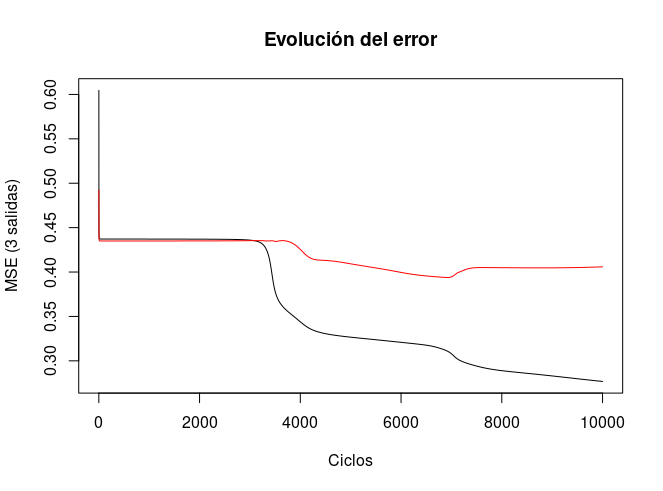
\includegraphics[width=.8\linewidth]{Images/best_fold1.png}
  \caption*{Hoja 1}

  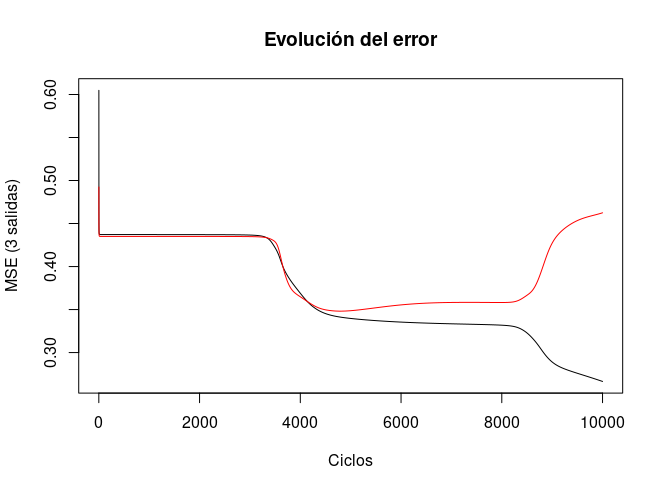
\includegraphics[width=.8\linewidth]{Images/best_fold3.png}
  \caption*{Hoja 3}
\end{minipage}%
\begin{minipage}{.52\textwidth}
  \centering
  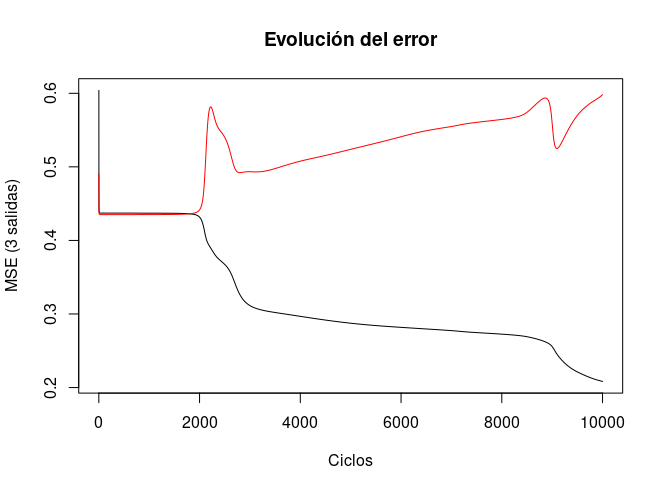
\includegraphics[width=.8\linewidth]{Images/best_fold2.png}
  \caption*{Hoja 2}

  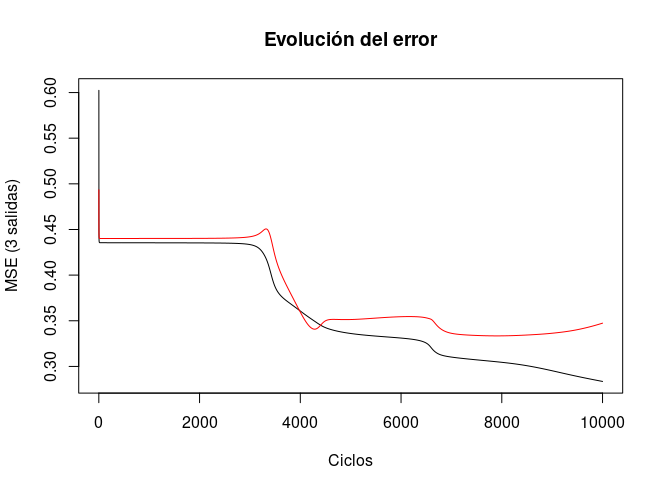
\includegraphics[width=.8\linewidth]{Images/best_fold4.png}
  \caption*{Hoja 4}
\end{minipage}
\end{figure}

Se observa claramente que, a pesar de que este sea el mejor experimento conseguido, sigue produciendo mucho sobreaprendizaje en el error. En algunos casos más grande que en otros.

\vspace{2mm}

Por ejemplo, la hoja 1 y la hoja 4 son las que sufren menor sobreaprendizaje. Mientras que la hoja 2 y la hoja 3 sufren más sobreaprendizaje, especialmente la 2.

\vspace{2mm}

A pesar de que estas medidas puedan no parecer demasiado buenas, no quiere decir que el modelo sea malo, porque el error no está directamente relacionado con el porcentaje de aciertos.



\subsection{Comparativa de los mejores experimentos}

Tal y como se mencionaba al principio de la sección de  \textit{Experimentación y análisis de los resultados}, la medida que se ha usado como determinante a la hora de decidir qué experimento es mejor que otro es el porcentaje de aciertos en el conjunto de test.

\vspace{2mm}

Por ello, se muestra en la siguiente gráfica una comparativa de estos resultados para los mejores experimentos:

\begin{figure}[!h]
\centering
  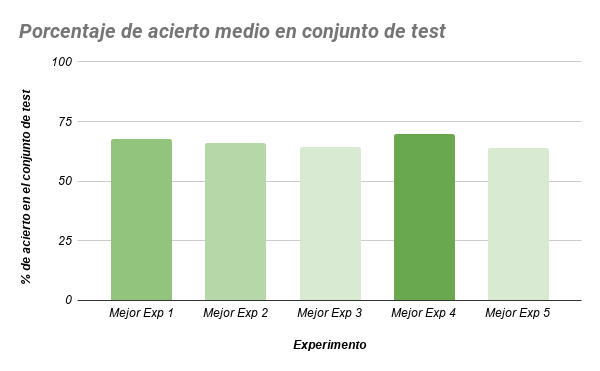
\includegraphics[width=.7\linewidth]{Images/p_acierto_medio_test.png}
  \caption*{Gráfica porcentaje de acierto medio en conjunto de test}
\end{figure}

Gracias a esta gráfica se puede ver cómo de buenos son los mejores experimentos obtenidos. Se ve que la diferencia entre el mejor (Mejor Exp. 4) y el resto no es muy grande, pues sus porcentajes son ligeramente menores.

\vspace{2mm}

A continuación se va a mostrar una gráfica comparativa de los resultados para cada experimento dividido por hojas, así como la media de hojas:

\newpage

\begin{figure}[!h]
\centering
  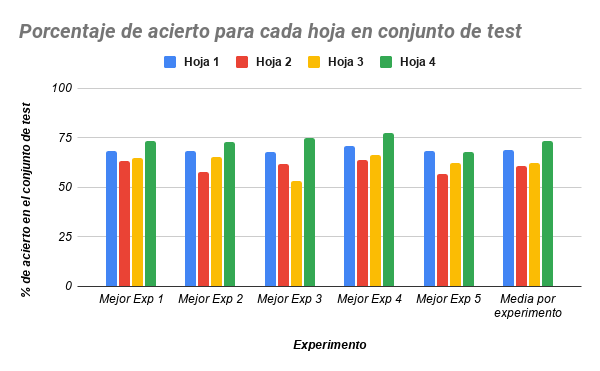
\includegraphics[width=.7\linewidth]{Images/p_acierto_cada_hoja_test.png}
  \caption*{Gráfica porcentaje de acierto para cada hoja en conjunto de test}
\end{figure}

Como se puede apreciar por los distintos experimentos, y se confirma con la media por experimento, la \textit{Hoja 2} es la que tiene más dificultad para clasificar correctamente a los individuos, mientras que la \textit{Hoja 4} es la que mejor lo hace.

\vspace{1mm}

Esto se debe a la generación y organización aleatoria de las hojas, que hacen que unas sean más diferentes respecto a los conjuntos de entrenamiento, y otras sean más similares.



\section{Conclusión}


La práctica ha permitido familiarizarse con los conceptos de validación cruzada estratificada, así como estudiar y analizar un modelo con clases desbalanceadas.

\vspace{2mm}

También permite profundizar en los métodos de experimentación y análisis en la resolución de modelos de Redes de Neuronas Artificiales.

\vspace{4mm}

Dado que las posibles combinaciones en la experimentación son muy grandes, se ha intentado abordar fijando el número de ciclos, y después modificando este número exclusivamente en los mejores experimentos. A pesar de que este no es el método ideal, es el que se ha decidido por limitaciones de tiempo y espacio en la memoria.

\vspace{2mm}

Por otro lado, el problema planteado ha permitido estudiar la clasificación de imágenes desde un punto de vista diferente a las arquitecturas de Redes de Neuronas Convolucionales.





\end{document}
